\section{Fases}

Nesta seção são apresentadas as descrições detalhadas das três fases do jogo.

\subsection{Fase 1}

Com nível de dificuldade baixo, a primeira fase representa a jornada de Medrash à tribo aliada Marakai pela floresta.

\subsubsection{Contextualização}

Após encontrar a sua tribo completamente destruída pelos guerreiros luskans, Medrash imediatamente começa uma jornada contra o tempo para tentar resgatar os membros de sua tribo -- que foram levados para serem escravizados -- antes deles chegarem na tribo Luskan. Medrash terá dois objetivos principais: chegar ao final da trilha deixada pelos guerreiros luskans e matar o tigre que o retardará de cumprir o objetivo anterior.

\subsubsection{Descrição do Espaço}

O espaço desta fase será uma floresta de coníferas. Esta será constituida de cinco regiões com suas próprias características : A, B, C, D e E, tal como esboçado no mapa da Figura \ref{fig:MapaDaFase1}. A região A, localizada na parte mais alta do mapa, é onde se encontra a tribo de Medrash e também é o ponto inicial do jogo. Para deslocar-se da região A à C, Medrash terá que passar obrigatoriamente pela região B, que é inclinada, cheia de rochas e infestada de cobras. A região C será plana e composta por muitas árvores. Esta área será dominada por ursos e em algumas ávores haverá cachos de abelhas. Na região D há um rio repleto de jacarés. Medrash poderá atravessá-lo andando (não correndo), já que as águas são baixas, ou pulando sobre as rochas no rio. Por fim, na reigão E, é onde encontra-se o último oponente de Medrash: o tigre. 

\begin{figure}[h]
\centering
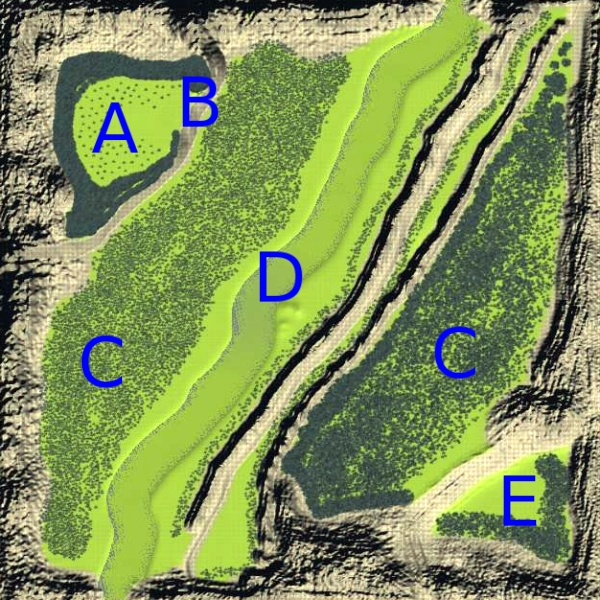
\includegraphics[width=10cm]{fases_mapa_1.jpg} 
\caption{Mapa da primeira fase}
\label{fig:MapaDaFase1}
\end{figure}

\subsubsection{Dificuldades ao Jogador}

As dificuldades de percurso serão as rochas soltas na descida da montanha onde esta localizada a tribo Ari, os cachos de abelhas espalhados pela floresta e as rochas sobre às águas do rio. As dificuldades de inimigos serão as cobras, ursos, jacarés e, no final, um tigre. O jogador também terá que administrar os medidores dos níveis de vitalidade e resistência física do Medrash, que estarão ativos nesta fase, exceto na etapa de enfrentamento do tigre, na qual apenas o primeiro estará ativo.

\subsubsection{Sequência dos Acontecimentos}

A seguir é apresentada a sequência dos acontecimentos da fase:

\begin{enumerate}
\item Uma animação ilustrará a chegada de Medrash à sua tribo Ari após uma longa caçada na mata. Ele encontrará seu amigo Gardain gravemente ferido em meio aos destroços da tribo. Gardain informará à Medrash o ocorrido e indicará o caminho que ele deverá seguir.
\item O jogador assume o controle de Medrash, que inicia com um porrete em mãos. Ele terá que seguir os rastros deixados pelos guerreiros invasores. Próximo à beira da montanha onde a tribo Ari está localizada, será possível avistar toda a floresta pelo qual Medrash deverá prosseguir.
\item Na descida da montanha haverão cobras e pedras soltas. Se Medrash cair, ele poderá morrer ou ficar gravemente ferido.
\item Após descer a montanha, Medrash estará em uma região plana dominada por ursos e cheia de cachos de abelhas.
\item Seguindo os rastros, Medrash chegará a um rio infestado de jacarés. Ele deverá atravesá-lo, seja andando pelas águas baixas ou saltando sobre as rochas.
\item Após a travessia, haverá continuidade dos rastros. Novamente haverá um região plana dominada por ursos e cheia de cachos de abelhas.
\item Próximo ao final da trilha, Medrash encontrará o corpo de um guerreiro morto. Junto a ele haverá uma lança, que o jogador poderá trocar pelo porrete.
\item No final da trilha haverá um tigre que impedirá a continuidade de Medrash. Ele deverá lutar com o tigre e matá-lo para finalizar a primeira fase.
\end{enumerate}

\subsection{Fase 2}

Com nível de dificuldade médio, a segunda fase representa a jornada de Medrash à tribo aliada Akanul pela montanha Kabalu.

\subsubsection{Contextualização}

Visando se adiantar à chegada dos guerreiros luskans na tribo Akanul -- última tribo aliada dos aris --, Medrash inicia uma jornada pela perigosa montanha Kabalu. Os objetivos principais de Medrash serão: cruzar a perigosa montanha a salvo e ajudar os guerreiros akanuls na defesa da tribo contra o ataque dos guerreiros luskans.

\subsubsection{Descrição do Espaço}

O espaço desta fase será a perigosa montanha Kabalu, que além de ser uma região de baixa temperatura, também é infestada de lobos selvagens. A Figura \ref{fig:MapaDaFase2} ilustra um esboço do mapa do local. A região A, representa a montanha Kabalu, cuja travessia é difícil, pois há fendas abertas no chão. E a região B representa a localização da tribo Akanul.

\begin{figure}[h]
\centering
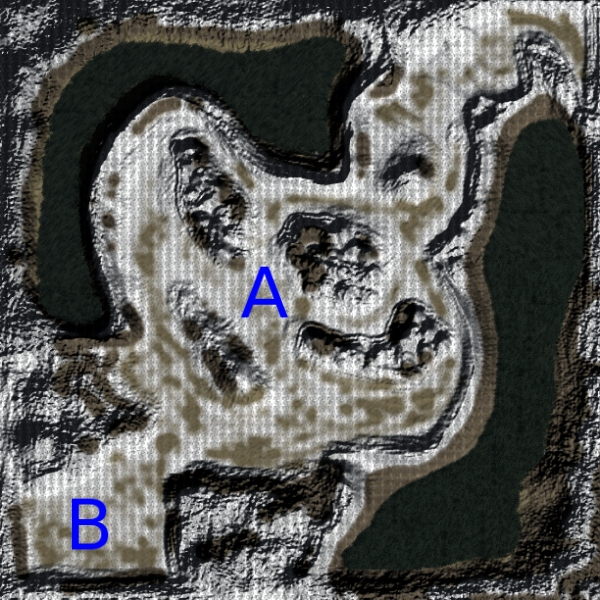
\includegraphics[width=10cm]{fases_mapa_2.jpg} 
\caption{Mapa da segunda fase}
\label{fig:MapaDaFase2}
\end{figure}

\subsubsection{Dificuldades ao Jogador}

As dificuldades de percurso serão as fendas abertas no chão e a baixa visibilidade do mesmo, já que o percurso será realizado de noite. As dificuldades de inimigos serão os lobos selvagens espalhados ao monte pela região e os guerreiros luskans que Medrash deverá infrentar no final da fase. O jogador também terá que administrar os medidores dos níveis de vitalidade e calor corpóreo do Medrash, que estarão ativos nesta fase, exceto na etapa de enfrentamento dos guerreiros luskans, na qual apenas o primeiro estará ativo.

\subsubsection{Sequência dos Acontecimentos}

A seguir é apresentada a sequência dos acontecimentos da fase:

\begin{enumerate}
\item Uma animação ilustrará Medrash avistando uma nuvem de fumaça ao longe. Ele correrá em direção a ela e verá os guerreiros luskans encerrando um forte ataque à tribo Marakai. Após a retirada dos lunkans, Medrash se aproximará da tribo e encontrará Rangrin gravemente ferido em meio aos destroços. Este o informará de que os luskans irão atacar a tribo Akanul e que Medrash deverá ir até ela pela montanha Kabalu para chegar antes deles.
\item O jogador assume o controle de Medrash. Medrash terá em mãos, além do porrete ou da lança, uma tocha acessa. Enquanto a tocha estiver acessa, os lobos não irão atacá-lo e a visibilidade do local próximo a ele será boa. Contudo, quando esta se apagar devido a rajadas de vento, os lobos perseguirão Medrash por toda região e a visibilidade das fendas no chão serão dificultosas. Medrash deverá acender a tocha em troncos de árvores atingidas por raios e ser rápido.
\item Ao atravessar a montanha, uma animação exibirá Medrash chegando à tribo Akanul e eles se preparando para o confronto.
\item O jogador novamente assume o controle de Medrash. Medrash terá em mãos um machado. Ele deverá proteger uma das moradias da tribo de guerreiros luskans que tentaram atear fogo nela.
\item Medrash deverá impedir que quatro desses guerreiros ateiem fogo na moradia para finalizar a fase.
\end{enumerate}

\subsection{Fase 3}

Com nível de dificuldade difícil, a terceira e última fase representa o contra-ataque dos guerreiros akanuls à tribo Luskan.

\subsubsection{Contextualização}

Como uma forma de retribuir à ajuda de Medrash, os guerreiros akanuls se unem ao herói e juntos partem em direção à tribo Luskan para contra-atacá-los. Já em território inimigo, enquanto os guerreiros akanuls e luskans confrontam-se, Medrash terá que cumprir dois objetivos: libertar os membros das tribos Ali e Marakai que foram capturados e aprisionados pelos guerreiros luskans; e enfrentar Balasar -- o temido líder dos luskans -- para resgatar a sua amada esposa Sora, que encontra-se aprisionada.

\subsubsection{Descrição do Espaço}

O espaço desta fase será o território da tribo Luskan. A Figura \ref{fig:MapaDaFase3} ilustra um esboço do mapa do local. A região A representa o local onde estarão as celas cujos membros das tribos Ari e Marakai estão aprisionados. A região B representa o local onde será o combate final entre Medrash e Balasar.

\begin{figure}[h]
\centering
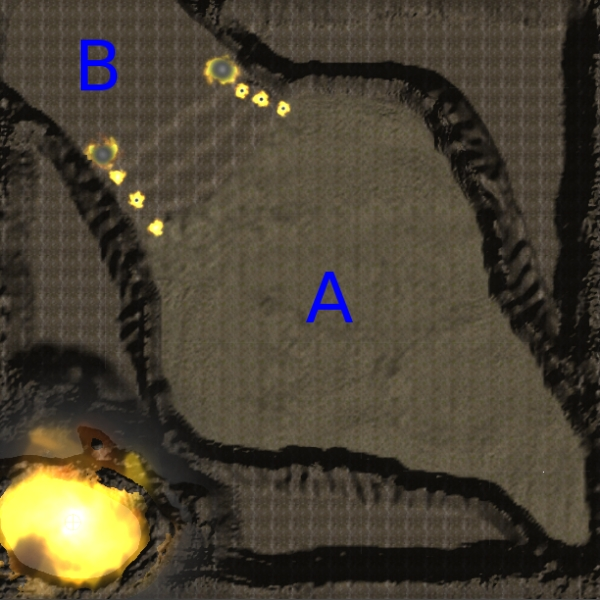
\includegraphics[width=10cm]{fases_mapa_3.jpg} 
\caption{Mapa da terceira e última fase}
\label{fig:MapaDaFase3}
\end{figure}

\subsubsection{Dificuldades ao Jogador}

As dificuldades de percurso serão as celas dos escravos e a lava do vulcão. As dificuldades de inimigos serão os guerreiros luskans, que impediram Medrash de libertar os membros das tribos, e Balasar. O jogador também terá que administrar os medidores do nível de vitalidade do Medrash e de tempo, que estarão ativos nesta fase, exceto na etapa de enfrentamento de Balasr, na qual apenas o primeiro estará ativo.

\subsubsection{Sequência dos Acontecimentos}

A seguir é apresentada a sequência dos acontecimentos da fase:

\begin{enumerate}
\item A fase começará com uma animação mostrando a chegada dos guerreiros akanuls e de Medrash no território dos luskans e o início do confronto.
\item O jogador assumirá o controle de Medrash, que encontra-se rodeado pelos combatentes, porém fora do alcance dos inimigos.
\item Assim que Medrash se aproximar demais de uma das três celas feitas de estacas de madeira, um guerreiro luskan ateará fogo na respectiva cela. O medidor de tempo será iniciado.
\item Outros guerreiros luskans irão atacar Medrash tentando impedí-lo de libertar os membros aprisionados.
\item Medrash precisará libertar os prisioneiros das três celas dentro do tempo para que possa prosseguir na fase. Se isto ocorrer, uma animação mostrará o vulcão entrando em erupsão e Balasar levando Sora para outro local. Medrash irá segui-lo. Ao chegar lá, Medrash verá sora aprisionada em uma cela.
\item O jogador assumirá novamente o controle de Medrash, que deverá enfrentar Balasar. Enquando ambos lutam, lava vulcânica irá escorrer para a direção de Sora. Medrash deve aproveitar enquando Balasar fica zonzo para bater nas estacas de madeira da cela.
\item Se Medrash conseguir destruir a cela há tempo que a lava não chegue até ela, então uma animação ilustrará Medrash aplicando um último golpe em Balasar, que cairá na lava. Por fim, ambos correm do local para ficarem a salvos do vulcão.
\end{enumerate}